





\documentclass[11pt,a4paper,final]{report}

\makeindex
\PassOptionsToPackage{nottoc}{tocbibind}

\usepackage{Packages/mathphdthesis}

\usepackage{acro}
\clearpage{}
\DeclareAcronym{2d}{
	short=2D,
	long=two-dimensional,
}
\DeclareAcronym{3d}{
	short=3D,
	long=three-dimensional,
}
\DeclareAcronym{a0}{
	short=A$_0$,
	long=antisymmetric fundamental Lamb wave mode,
}
\DeclareAcronym{ccd}{
	short=CCD,
	long=correlation coefficient deviation,
}
\DeclareAcronym{cfrp}{
	short=CFRP,
	long=carbon fibre reinforced polymer,
}
\DeclareAcronym{cpu}{
	short=CPU,
	long=central processing unit,
}
\DeclareAcronym{di}{
	short=DI,
	long=damage index,
	plural-form=damage indices,
}
\DeclareAcronym{dau}{
	short=DAU,
	long=data acquisition unit,
}
\DeclareAcronym{dof}{
	short=DOF,
	long=degree of freedom,
	plural-form=degrees of freedom,
}
\DeclareAcronym{emi}{
	short=EMI,
	long=electromechanical impedance,
}
\DeclareAcronym{fem}{
	short=FEM,
	long=finite element method,
}
\DeclareAcronym{fbg}{
	short=FBG,
	long=fibre Bragg grating,
}
\DeclareAcronym{fgm}{
	short=FGM,
	long=full geometry model,
}
\DeclareAcronym{gw}{
	short=GW,
	long=guided wave,
}
\DeclareAcronym{gll}{
	short=GLL,
	long=Gauss-Lobatto-Legendre,
}
\DeclareAcronym{gpu}{
	short=GPU,
	long=graphics processing unit,
}
\DeclareAcronym{hsc}{
	short=HSC,
	long=honeycomb sandwich composite,
}
\DeclareAcronym{lm}{
	short=LM,
	long=Lagrange multipliers,
}
\DeclareAcronym{ncn}{
	short=NCN,
	long=National Science Centre,
}
\DeclareAcronym{madif}{
	short=MADIF,
	long=model-assisted damage identification function,
}
\DeclareAcronym{mapd}{
	short=MAPD,
	long=mean-absolute-percentage deviation,
}
\DeclareAcronym{pnn}{
	short=PNN,
	long=probabilistic neural networks,
}
\DeclareAcronym{pzt}{
	short=PZT,
	long=piezoelectric transducer,
}
\DeclareAcronym{rms}{
	short=RMS,
	long=root-mean-square,
}
\DeclareAcronym{rmsd}{
	short=RMSD,
	long=root-mean-square deviation,
}
\DeclareAcronym{rve}{
	short=RVE,
	long=representative volume element,
}
\DeclareAcronym{s0}{
	short=S$_0$,
	long=symmetric fundamental Lamb wave mode,
}
\DeclareAcronym{sem}{
	short=SEM,
	long=time domain spectral element method,
}
\DeclareAcronym{scs}{
	short=SCS,
	long=sandwich composite structure,
}
\DeclareAcronym{shm}{
	short=SHM,
	long=structural health monitoring,
}
\DeclareAcronym{sldv}{
	short=SLVD,
	long=scanning laser Doppler vibrometer,
}
\clearpage{}
\usepackage[ruled,vlined]{algorithm2e}
\usepackage{multirow}
\graphicspath{{Figures/}} 

\includeonly{
Frontbackmatter/prelude 	,Frontbackmatter/newcom 	,Nomenclature/nomenclature  ,Acronyms/acronyms			,Chapters/Intro/intro  	    ,Chapters/Chapter2/ch:problem 	,Chapters/Chapter3/ch:method 	,Chapters/Chapter4/ch:sem 		,Chapters/Chapter5/ch:simulation 	,Chapters/Chapter6/ch:validation 	,Chapters/Chapter7/ch:tempEffect 	,Chapters/Chapter8/ch:severity 	,Chapters/Chapter9/ch:conclusions	,Appendices/app0   			,index  					}

\begin{document}

\clearpage{}

\titlepgtrue 												\signaturepagetrue 											\copyrighttrue 												\abswithesistrue 											\acktrue 													\tablecontentstrue 											\tablespagetrue 											\figurespagetrue 											

\title{Modelling of sandwich plates and piezoelectric transducers to identify the severity of mechanical damage}							\author{Piotr Fiborek} 	\prevdegrees{M.Sc. Eng.}              			\institute{Mechanics of Intelligent Structures Department}								

\submittedfor{A dissertation submitted to the Scientific Board of the Szewalski Institute of Fluid Flow Machinery, Polish Academy of Sciences in partial fulfillment of the requirements for the Degree of Doctor of Philosophy}			\advisor{ Pawe\l{} Kudela, D.Sc. Ph.D. Eng.} \dept{The Szewalski Institute of Fluid Flow Machinery, Polish Academy of Sciences}
\submitdate{June, 2022}						

\newcommand{\abstextwithesis}
{
...
}

\newcommand{\acknowledgement}
{
}

\newcommand{\engineeringquote}
{
\null\vskip1.8in
\begin{quote}
"Engineering ."\begin{flushright}- aaa 
\end{flushright}
\end{quote}
}

\renewcommand{\bibname}{References/Bibliography}
\setlength\bibitemsep{1.5\itemsep}

\newcolumntype{L}[1]{>{\raggedright\let\newline\\\arraybackslash\hspace{0pt}}m{#1}}
\newcolumntype{C}[1]{>{\centering\let\newline\\\arraybackslash\hspace{0pt}}m{#1}}
\newcolumntype{R}[1]{>{\raggedleft\let\newline\\\arraybackslash\hspace{0pt}}m{#1}}

\beforepreface
\afterpreface
\clearpage{}
\clearpage{}

\newtheorem{theorem}{Theorem}[section]
\newtheorem{lemma}[theorem]{Lemma}
\newcommand{\bfx}{{\ensuremath{\mathbf{x}}}}
\clearpage{}
\clearpage{}

\chapter*{NOMENCLATURE}
\addcontentsline{toc}{chapter}{NOMENCLATURE}
\label{nomenclature}



\nomtypeG{\( \lambda \)}{Full scale to model scale ratio}{$\frac{L_{s}}{L_{m}}$}{-}
\nomtypeG{\( \delta \)}{Boundary layer thickness}{-}{m}
\nomtypeG{\( \rho \)}{Mass density}{-}{kg/m\textsuperscript{3}}
\nomtypeG{\( \nu \)}{Kinematic viscosity}{$\frac{\mu}{\rho}$}{m\textsuperscript{2}/s}
\nomtypeG{\( \mu \)}{Viscosity}{$\frac{\mu}{\rho}$}{kg/ms}



\nomtypeD{\( \xi, \eta, \zeta \)}{local coordinates}{-}
\nomtypeD{\( w \)}{weighting factor}{$\frac{2}{p(p-1)\left(P_{p-1}(\xi)\right)^2}$}


\nomtypeR[AN]{A\textsubscript{N}}{Nozzle discharge area}{-}{m\textsuperscript{2}}
\nomtypeR[AS]{A\textsubscript{S}}{Cross sectional area at station $s$}{-}{m\textsuperscript{2}}
\nomtypeR[SS]{S\textsubscript{S}}{Wetted surface area}{-}{m\textsuperscript{2}}

\nomtypeR[T]{T}{Draft}{-}{$m$}
\nomtypeR[LOA]{L\textsubscript{OA}}{Length overall}{-}{m}
\nomtypeR[LWL]{L\textsubscript{WL}}{Length waterline}{-}{m}
\nomtypeR[B]{B}{Moulded breadth}{-}{m}
\nomtypeR[Bhullm]{B\textsubscript{hull, m}}{Beam of model hull}{-}{m}

\printnomenclature[6em]
\clearpage{}
\clearpage{}

\chapter*{ACRONYMS}
\addcontentsline{toc}{chapter}{ACRONYMS}
\label{acronyms}
\printacronyms[heading=none,pages={display=first}]\clearpage{}
\clearpage{}\pagenumbering{arabic}



\chapter[Introduction]{Introduction}
\label{ch:intro}
The dissertation results from the author’s work as an assistant in the Department of Mechanics of Intelligent Structures, Institute of Fluid Flow Machinery, Polish Academy of Sciences.
Most of the work has been carried out within the framework of a research project titled ‘Model-assisted damage identification function for Structural Health Monitoring of composite structures under a varied environmental condition', which was granted to the author by the National Science Centre, Poland.
The primary objective was to develop a new approach to a sandwich structure assessment based on guided waves techniques under varied operating conditions.
The essence of the proposed method is to establish an accurate and numerically efficient model of the wave propagation in the sandwich structure to determine the severity of the damage.
A better understanding of guided wave behaviour in such structures and their interaction with damage will help develop more precise structural health monitoring strategies, reducing costs without compromising the safety of the liable systems.


\section{Sandwich Composite Structures}
\label{sec:scs}

Composites consist of two or more different materials, such as plastics, resins, metal alloys, glass, carbon or bio-based fibres. The combination gives  structure benefits from the properties of the component materials, e.g., the strength of carbon fibres and the low density of the polymer resin in the case of \ac{cfrp}.
The contribution of lightweight composite materials to the production of structural components has been increasing rapidly since the middle of the last century.
Due to the high strength-to-weight ratio, higher operating temperatures, greater stiffness and higher
reliability, composite materials are extensively used in the aircraft and aerospace industry and civil constructions.
Composites account for more than 50\% of the total weight of the aircraft Boeing B787 and Airbus A350 \cite{giurgiutiu2015structural}.

One group of composites includes sandwich panels, which is a type of multi-layered structure that are composed of the mid-core sandwiched between thin skins.
The skins, made of high strength materials, are designed to carry tensile or compressive stresses from longitudinal forces and bending moments.
On the other hand, the core transmits mainly shear stresses from transverse forces.
It also separates the skins, which increases structural stiffness for thin layers, improves insulation properties, and reduces weight while maintaining strength properties similar to the solid construction of the same density.
A popular core used in engineering structures is a honeycomb geometry core.
Fig.~\ref{fig:hcp} shows the construction of the \ac{hsc}.
The core can be made of aluminium, cardboard or Nomex. 
\begin{figure}[H] \begin{center}
		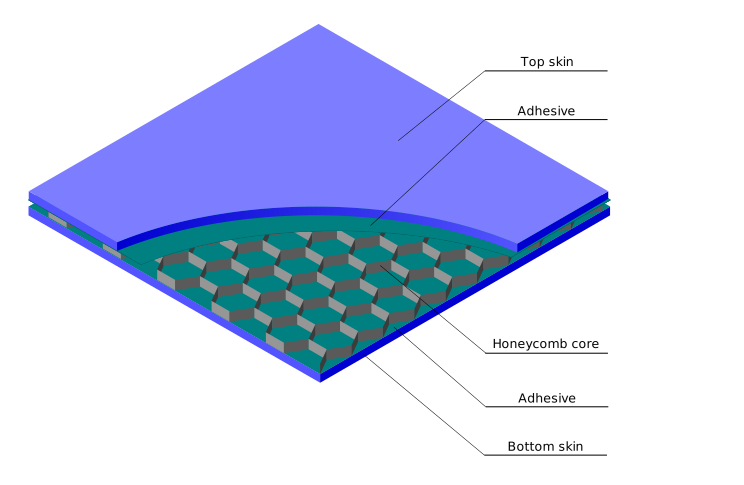
\includegraphics[width=1\linewidth]{Intro/honeycomb_plate}
		\caption{
			\label{fig:hcp} Structure of the honeycomb sandwich composite.}
		\vspace{-0.5cm}
	\end{center}
\end{figure}

However, these complex structures are exposed to various types of damage that are not found in metal alloy materials, e.g., hidden disbonds between the skin and the core, delamination of the composite skins, or the core impact damage.
They can occur either during a manufacturing process, storage or in-service life.
Therefore, advanced methods are required for online damage detection.
Thus, the use of composites has forced the development of progressive approaches to structural inspections. \section{Structural Health Monitoring}
\label{sec:scm}

\Ac{shm} is the process of implementing an advanced damage identification strategy for structural or mechanical systems \cite{farrar2007introduction}.
The \ac{shm} systems usually consist of a sensor network, a \ac{dau}, and a central processor.
The \ac{dau} is responsible for collecting the data measured by the sensor network and the intact structure data if used \ac{shm} technique requires it.
A central unit then determines the current state of the structure through signal processing and statistical classification.
The implementation of \ac{shm} aims to extend the safe life of the monitored system, or usage of lightweight materials, which leads to cost reduction in production and operation.
For example, composites and adhesive bonding techniques reduces the aircraft's overall weight, reducing fuel consumption \cite{scelsi2011potential}.
\ac{shm} is most commonly found in structures, such as aerospace, civil and mechanical engineering, where damage can have catastrophic consequences.

Rytter, in his dissertation \cite{rytter1993vibrational}, classified the \ac{shm} system advancement into the following four levels:
\begin{itemize}
	\item[] \textbf{Level 1}: Detection.
	\item[] \textbf{Level 2}: Localization.
	\item[] \textbf{Level 3}: Assessment.
	\item[] \textbf{Level 4}: Consequence.
\end{itemize}
The first level determines if any adverse change in the geometric has occurred or material characteristics of the system. The second level leads to the localization of the damage.
The third and fourth level systems determine the size of the flaw and decide whether any maintenance is necessary, respectively.
The existence and location of faults can be defined in unsupervised learning mode by taking a threshold value for a measurable, damage-sensitive system feature. The threshold should be compensated depending on the prevailing operational and environmental conditions.
In contrast, damage size is determined in supervised learning mode based on an analytical model or data extracted experimentally from the structure \cite{worden2007fundamental}. \section{Piezoelectric Transducers}
\label{sec:PZT}

The piezoelectric phenomenon is the generation of an electrical charge on the surface of materials under mechanical deformation in crystalline materials with no inversion symmetry.
The magnitude of the generated charge is proportional to the strain and the direction of polarization.
Those materials also exhibit the opposite effect: a change in size due to an applied electric field.
Piezoelectric materials are widely used in engineering as electroacoustic transducers, high voltage generators and power sources, energy harvesters, micro motors and actuators.
\begin{figure}[H]
\includegraphics[width=1\linewidth]{Intro/PZTs}
\caption{Various types of piezoelectric transducers \textbf{(a)} circular discs, \textbf{(b)} circular array of the transducers, \textbf{(c)} Smart Layer\textsuperscript{\tiny\textregistered} - piezoelectrics embedded into dielectric film.}
	\label{fig:piezo}
\end{figure}
\Acp{pzt}, the acronym derived from the chemical formula of the most commonly used piezoelectric ceramic, i.e. Pb[Zr\(_x\)Ti\(_{1-x}\)]O\(_3\) (lead zirconate titanate), are lightweight, various size and shape structures. 
They can be permanently mounted on the structure surface, embedded within the material, or even be a smart composite material.
In \ac{shm}, they are mainly used in elastic wave propagation, modal analysis, and \ac{emi} methods. \section{Chosen \ac{shm} techniques using \acp{pzt}}
\label{sec:techniques}



\subsection{Guided waves based techniques}


\Acp{gw} are mechanical vibrations being a superposition of shear and longitudinal waves propagating in a bounded elastic medium, e.g., bars, beams, rods, plates and shells. 
Guided waves are multi-modal and dispersive, i.e. more than one mode travels simultaneously through the medium with the phase velocity depending on the frequency.
Fig.~\ref{fig:dispersion} shows an example of dispersion curves generated by the Dispersion Calculator~\cite{huber2021dispersion} software tool for a 1 mm thick \ac{cfrp} plate in the frequency range 0-2000 kHz.
\Ac{a0} and \ac{s0}, considering the distribution of particle displacements on the upper and lower free surface relative to a central surface, are observed for low frequencies.
The mode shapes are pictured in Fig.~\ref{fig:mode_shape}, with the \ac{s0} particle displacements being dominant in-plane, while the \ac{a0} is dominated by out-of-plane.
Moreover, higher harmonic modes appear over the cut-off frequency, as shown in Fig.~\ref{fig:dispersion}.
\begin{figure}
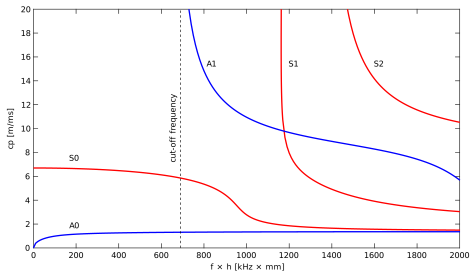
\includegraphics[width=1\linewidth]{Intro/dispersion}
\caption{Dispersion diagram for a 1 mm \ac{cfrp} plate (adopted from Dispersion Calculator~\cite{huber2021dispersion}). Red and blue solid curves represent symmetric and antisymmetric modes, respectively; a black dashed line indicates the cut-off frequency for higher modes.}
	\label{fig:dispersion}
\end{figure}
\begin{figure}
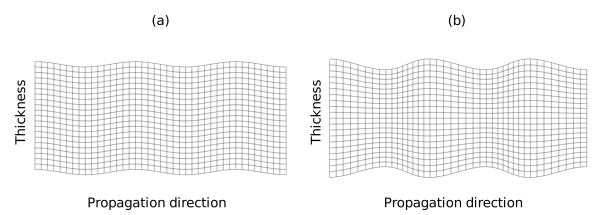
\includegraphics[width=1\linewidth]{Intro/mode_shape}
\caption{Mode shape of the \textbf{(a)} \ac{a0} and \textbf{(b)} \ac{s0} at 100 kHz for \(\phi=0^{\circ}\) in 2 mm composite plate (exported from Dispersion Calculator~\cite{huber2021dispersion}).}
	\label{fig:mode_shape}
\end{figure}

Detection schemes based on \acp{gw} exploit reflection, attenuation, and mode conversion when the propagating wave encounters a discontinuity in the structure \cite{alleyne1992interaction}.
Thus, this technique is efficient in detecting various types of defects, such as delamination \cite{sohn2011delamination,tian2015delamination}, adhesive disbonds \cite{rucka2018damage,balasubramaniam2021ultrasonic}, corrosion changes \cite{alleyne1995long,lowe1998defect}, cracks \cite{tua2004detection,lu2006crack,zima2020detection} and failures occurring in \acp{hsc} \cite{mustapha2011assessment, sikdar2016guided, sikdar2016ultrasonic,radzienski2016assessment, yu2019core}.
Many techniques based on \ac{gw} propagation have been developed for damage detection and localization.
A pitch-catch technique \cite{ihn2008pitch, sikdar2017structural} uses a pair of detached sensors, one excites, and the other receives a signal.
If the wave encounters a defect between the sensors, it will scatter, and the recorded signal will be distorted.
In the case of the pulse-echo technique \cite{guo1993interaction, kudela2008damage}, there is one sensor that excites the wave and, at the same time, registers possible echoes from the damage.
The damage localization can be determined if the wave speed is known and the time of flight is measured.
The radar principles were utilized in a phased array technique for plate inspection \cite{giurgiutiu2004embedded, ostachowicz2008elastic, kudela2018structural}.
The technique uses an array of transducers, each excited with an appropriate time offset, to focus all the waves at a single grid point of the area to be inspected.
A damage map is determined once the signals are obtained and processed for the entire grid.
Fink proposed a different approach, developing what he called a time-reversal mirror \cite{fink1992time}.
In this method, the wave propagates from one sensor to another, and then after time-reversal and dispersion compensation, the wave is re-emitted to the origin sensor.
The resulting signal will be a mirror image of the forcing signal only if the wave does not encounter damage along the way \cite{park2007time, eremin2016analytically}.

The \acp{pzt} can be used mutually as actuator-receiver pairs or as a single actuator with other types of devices, e.g. \ac{sldv}, \ac{fbg} sensors.
The \acp{pzt} generate high forces with broadband frequency, so methods based on \ac{gw} can detect various damage types of different sizes in a large inspected area.
Moreover, specific algorithms do not require a baseline model, and the method implementation is economically efficient.

\subsection{Electromechanical impedance methods}
\Ac{emi} spectroscopy is also an effective and powerful technique in \ac{shm} for real-time structural damage assessment \cite{park2003overview}.
The basis of this method is the influence of the mechanical impedance of the inspected host structure on the electrical impedance of the \ac{pzt} attached to the structure.
Assuming that the mechanical property of the sensor remains unchanged over the monitoring period, any changes in measurements of the electrical impedance can be considered a difference in the structure stiffness, which in turn can indicate that a defect has occurred.

Fundamentals of the \ac{emi} method were introduced by Liang et al. \cite{liang1994impedance}.
An analytical model of a \ac{pzt} actuator bonded to one end of a single degree of freedom mass-spring-damper system was presented in this pioneering work.
In the early papers, the authors adopted quasi-static sensor approximation until  Giurgiutiu and Zagrai \cite{giurgiutiu2000characterization} derived an expression where the sensor dynamic was incorporated.
The dynamics of a single \ac{pzt} with various boundary conditions (free, clamped and elastically constrained) and sensor attached to a beam were considered.
Further investigation was performed for the sensor bonded to the host structures was performed \cite{zagrai2001electro, giurgiutiu2005damage}.
Damage detection is realized by comparing the state of the structure with the reference state using overall statistical damage indices, e.g., the \ac{rmsd}, the \ac{mapd}, \ac{ccd} and \ac{pnn}.
Malinowski et al. \cite{malinowski2014characterisation, malinowski2015use} investigated the effects of \ac{emi} changes related to the state of the adhesive layer between two composite plates.
The technique has been used to evaluate weak bonds due to inadequate adhesive curing temperature, release agent and moisture contamination. This type of damage is not detectable using the method based on \ac{gw} propagation.
Experimental testing was conducted on weakened samples and compared with a reference.
The \ac{rms} of the conductance in the range of 3-5 MHz and the first thickness resonant frequency shift were considered for bond-line assessment.

An and Sohn \cite{an2012integrated} proposed a new damage detection technique that combines \ac{emi} and \ac{gw} advantages.
In the method, measured admittance characteristic is separated into two parts: active and passive.
\Ac{di} is a weighted sum of two indicators obtained from \ac{gw} signal and active admittance.
Because passive impedance is only sensitive to temperature variation, it is used for temperature compensation on both mentioned signals.
Instead of two \acp{di}, Sevillano et al. \cite{sevillano2016damage} proposed more integrated \ac{di} based on the electromechanical power dissipation of the \ac{pzt} sensor.

The \ac{emi} technique can detect damage, such as delamination or cracks, but is also sensitive to changes, such as weak bonds, which the \ac{gw} method is ineffective at detecting.
However, the \ac{emi} is a local method for the high frequency.
Giurgiutiu et al. \cite{giurgiutiu2001electro} obtained consistent results for crack detection in distances up to 40 mm in the frequency range 300-450 kHz. 
This method is also sensitive to environmental conditions such as temperature and humidity fluctuations\cite{bhalla2002practical} or loading variations \cite{lim2011impedance}.

%
 \section{Challenges in Damage Assessment in the \ac{hsc}}
\label{sec:challenges}

The assessment of the damage magnitude in structural materials requires the development of a database of the effect of damage on system response \cite{worden2007fundamental}.
In the case of \ac{hsc}, many factors affect the \ac{di} magnitude, such as damage localization, material properties and dimensions, the sensor position relative to the core cell and the boundary conditions.
Considering all the factors, the determination of DI by experimental means becomes very complicated, expensive and time-consuming.
Therefore, numerical analysis and computer simulations become the only practical tool to achieve the goal.

The most common \ac{hsc} numerical model used in analysing \acp{gw} and \ac{emi} found in the literature is the model based on the \ac{fem}.
Although the numerical results are consistent with the experimental results, the models have some limitations in performing the simulations in a reasonable computation time and operating memory consumption.
The improvements include:
\begin{itemize}
\item reduction of the sample dimensions \cite{hosseini2013numerical, tian2015wavenumber};
\item homogenisation of the core properties \cite{catapano2014multi, zhou2020debonding};
\item a simplified \ac{2d} model based on a cross-section of the panel \cite{li2019detection};
\item neglect of an adhesive layer \cite{mustapha2013non}.
\end{itemize}
The time and memory consumption of the FEM simulations is due to the high spatial resolution needed to converge the numerical results.
When first-order elements are used, up to twenty nodes per the shortest wavelength of interest is recommended by Moser et al. \cite{moser1999modeling}.
Therefore, implementations with higher-order elements have been developed in recent years, achieving convergence even at six nodes \cite{willberg2012comparison}.
One is a method based on Lagrange polynomials as a shape function and \ac{gll} for integration scheme, termed \ac{sem}.
The \ac{sem} has initially developed for the numerical solution of the fluid flow in a channel by Patera \cite{patera1984spectral}. The method has also been successfully employed for elastic wave propagation by many researchers \cite{seriani1994spectral, kudela2007wave, ostachowicz2011guided, rucka2010experimental, schulte2011simulation, lonkar2014modeling, rekatsinas2017cubic, yu2020time, li2021hybrid}.

Due to the fast convergence and flexibility of the \ac{sem}, Kudela applied the method to model \ac{hsc} with full core geometry.
Despite the small size of the plate ($179 \times 159$ mm), the model has more than 1.5 million \acp{dof} because the skins and the core are composed of 3D elements.
The model size could be reduced if the shell element replaced the solid one.
In addition, the surface-mounted \ac{pzt} is omitted in the above model, and a concentrated force is used as the disturbance source.
The sensors mesh would have to coincide with the plate mesh or use the coupling between both meshes to include the \acp{pzt} in the simulation.
Such coupling can be realized using an interface based on Lagrange multipliers proposed by Farhat and Roux for domain decomposition in \ac{fem} \cite{farhat1991method}.
Ashwin et al. implemented the interface for the \ac{sem} but did not adopt it to non-matching grids \cite{ashwin2014formulation}, which is required for model generalization.

The efficient model and the computational hardware play a significant role in the simulation speed. 
Kudela presented the \ac{sem} algorithm for parallel calculation on the \ac{gpu} in the paper mentioned above.
The multi-core architecture of the \ac{gpu} enables simultaneous vector operations, making simulations over 14 times as fast as those performed by a \ac{cpu}.
Therefore, using the card will make it more convenient to perform simulations of models with numerous \acp{dof} to determine the effect of damage size on system response.
 \section{Conclusions}
\label{sec:conclusionsIntro}

In the Introduction, a brief overview of the issues undertaken in the dissertation has been presented,  i.e., composite materials, construction and their applications;  definition of the \ac{shm} and application of \ac{pzt} sensors in damage detection; and challenges in severity damage assessment in \acp{hsc}.
The literature review revealed the need for a practical tool failure estimation to fully exploit composites advantages in engineering structures. \clearpage{}
\clearpage{}



\chapter[Problem Statement]{Problem Statement}
\label{ch:problem}





Composite materials are used as structural components whose failure can have catastrophic consequences.
Although \ac{gw} based methods are promising for damage identification and localization, they have not been widely reported to estimate the failure size.
A better understanding of the effect of damage on elastic wave propagation in \acp{hsc} will allow the development of robust and practical tools to evaluate this structure.

The principal aim of this dissertation was to propose a new approach for the severity of damage identification in the \ac{hsc} employing the \ac{pzt} sensors.
The essence of the method is the determination of damage influence function on characteristic parameters of the propagating waves in the structure.
This function was defined using a numerical model developed by the \ac{sem}.

Initially, the model is prepared for the pristine sample under various operating conditions such as ambient temperature.
Then parametric simulations for different damage scenarios are performed.
The \ac{madif} is determined based on the obtained results. 
This function determines the flaw size depending on the \acp{pzt} response.
Damage is considered to be a debonding between the core and the skin. 
The following objectives of the dissertation are:
\begin{itemize}
	\item Develop a robust and efficient numerical model of the propagating \ac{gw} in the \ac{hsc} under varying ambient temperatures.
	\item Validate the model experimentally.
	\item Determine the \ac{madif} to define damage influence on the propagating waves.
	\item Investigate the structure experimentally under varied temperature conditions.
	\item Propose a framework of damage detection based on the \ac{madif}.
\end{itemize}

The imposed objectives lead to the proof of the thesis that it is possible to determine the function of damage severity in \acp{hsc} by numerical simulations.

Chapter \ref{ch:method} presents the methods for developing a model-assisted damage severity assessment scheme.

Chapter \ref{ch:sem} gives a theoretical background of the \ac{sem} for \ac{gw} propagation.
It includes mass, stiffness and damping matrices for 2D and 3D formulation; interface coupling algorithm; time integration scheme; and parallel implementation for GPU calculation.

Chapter \ref{ch:simulation} provides the details of the sample configuration for the full geometry and homogenized core models. The individual sample component grids, the signal parameters, and the damage model are presented.

The simulations and experimental validation results are presented in Chapter \ref{ch:validation}.

Chapter \ref{ch:tempEffects} includes the analysis of the GW propagation under variable temperature conditions.

The crucial part of the dissertation appears in Chapter \ref{ch:severity}. Based on the simulations performed and their validation experimentally, the function of the damage size effect on the elastic wave propagation in \ac{hsc} is revealed, termed \ac{madif}.

The conclusion of the dissertation and final remarks are provided in Chapter \ref{ch:conclusions}.

\clearpage{}
\clearpage{}

\chapter[Concept of the Method]{Concept of the Method}
\label{ch:method}






\section{Modeling of the GW Propagation in the \acp{hsc}}
\label{sec:modelling}





In the dissertation, the \ac{hsc} composed of an aluminium honeycomb core and the skins made of \ac{cfrp} is assumed for further analysis.
The most common numerical modeling of the phenomenon of \ac{gw} in \acp{hsc} found in the literature is a calculation of the effective material properties of the honeycomb structure \cite{baid2015dispersion, mustapha2014leaky, qi2008ultrasonic,  shi1995derivation, sikdar2016guided}.
The properties are obtained from the analytical \cite{gibson1982mechanics, malek2015effective} or \ac{fem} \cite{catapano2014multi, chen2014analysis} analysis of the honeycomb \ac{rve}.
A comprehensive literature review on the homogenisation of the honeycomb structure is presented in the work of Ahmed \cite{ahmed2019homogenization}.
Replacing the core geometry with a homogeneous material has many advantages.
First and foremost, it simplifies the domain mesh so that convergence of the solution requires fewer working memory resources and increases the value of the critical time step.
In addition, the wave propagation velocity determined by the simulation is in good agreement with the experiment.

However, this method cannot adequately represent the phenomenon of propagating wave interaction in honeycomb cells.
It causes the signal energy not to dissipate as it would in a real structure.
A more precise model is the \ac{fgm} of the core. 
Ruzzenne et al. presented a parametric study to evaluate the dynamic behavior of the honeycomb and cellular structures through the \ac{fem} and the application of the theory of periodic structures \cite{ruzzene2003wave}.
Recently, the simulations of the wave propagation in the \acp{hsc} have been conducted with commercially available finite element code~\cite{song2009guided, hosseini2013numerical, tian2015wavenumber, zhao2018wave}.

While the \ac{fem} based modelling of \ac{gw} requires a significant amount of memory and is time-consuming, this method becomes inefficient in the case of \ac{fgm}.
Kudela increased the computational efficiency with the model based on the time-domain \ac{sem} \cite{kudela2016parallel}.
In addition, the algorithm has been adapted for parallel computing on the \ac{gpu}, making the simulations fourteen times as fast as on the \ac{cpu}.
However, this approach has two major drawbacks. One is employing solid elements with three \acp{dof} at each node to model the core walls. As a result, a $179\times160$ mm sandwich panel has over 1.5 million \acp{dof}.
Secondly, no \ac{pzt} sensors were considered in the simulation, so a concentrated force was used to generate the \ac{gw}.
To attach the transducers, the grids of the sensor and the host plate must coincide or use an interface between them. 

The disadvantages mentioned above were motivation to propose a new model of the \ac{hsc}.
In the proposed model, the core of the plate consists of \ac{2d} elements, one per cell wall.
Since the neutral plane of the elements is oriented differently concerning the global coordinate system, the local displacements vector has to be transformed accordingly.
The skin model will be developed according to the laminate theory presented by Vinson and Sierakowski \cite{vinson1993behavior}.
In addition, two interfaces are used to connect the individual \ac{hsc} components.
One with the non-matching grid was developed to join the sensors with the panel.
It was done with the novel method based on the element shape function described in Chapter \ref{ch:sem}.
The core and skin connection was implemented with a perfect matching interface.
To the best of the author's knowledge, the presented model has not been implemented yet for the \acp{hsc}.

The parametric study conducted in the paper leads to the determination of a \ac{madif}, which defines the influence of the size of the composite defect on wave propagation.
In this case, the defect is assumed to be a disbond between the skin and the core. \section{Temperature Effect on the GW Propagation}
\label{sec:temp}



The measurements of \acp{gw} are within a range of milliseconds.
The temperature changes of the inspected structure within that period are negligible.
Therefore, \ac{gw} propagation can be modelled for the stationary temperature field.
It is assumed that the temperature field can be obtained from temperature sensors at the moment of \ac{gw} excitation.
A uniform temperature field was assumed in the model for simplicity.

In order to carry out the temperature-dependent \ac{sem} simulations, only changes in the elastic modulus of the \ac{hsc} components are considered.
The density changes are neglected. For the \ac{cfrp} skin, the modulus is calculated as per the methodology described in \cite{chamis1983simplified,salamone2009guided}.
The significant changes in mechanical properties under temperature occur mainly in the polymer matrix, while the variation in the carbon fibre properties has a negligible effect on wave propagation.
In this model \cite{salamone2009guided,hopkins2012extreme}, the reduction of Young’s modulus of the resin \(E_m\) with temperature variation is assumed as:
\begin{eqnarray}
	E_m(T)=F_m E_{rm},
	\label{eq:factor_temp}
\end{eqnarray}
where \(E_{rm}\) is the Young’s modulus of resin at the reference temperature and \(F_m\) is the temperature degradation factor as proposed in \cite{chamis1983simplified}:
\begin{eqnarray}
F_m=\sqrt{\frac{T_{g0}-T}{T_{g0}-T_r}},
\label{eq:em_temp}
\end{eqnarray}
where \(T_{g0}\) is the glass transition temperature and \(T_r\) is the reference temperature.
Equation \ref{eq:em_temp} is also applicable to determine the elastic modulus of the adhesive layer bonding the core to the skins, while for aluminium, the linear temperature dependence given by Hopkins et al. \cite{hopkins2012extreme} as:
\begin{eqnarray}
	E_a(T)=-\num{4e7}T+\num{8e10}.
	\label{eq:aluminium_temp}
\end{eqnarray}
The Young modulus and Poisson ratio of the sensors are in the form proposed by Lanza et al. \cite{lanza2008temperature}:
\begin{eqnarray}
	Y_{pzt}(T)=Y_{pzt}(T_r) + \num{16e7}(T_r-T),\\
	\nu_{pzt}(T)=\nu_{pzt}(T_r) + \num{13e-3}(T_r-T).
	\label{eq:pzt_temp}
\end{eqnarray}
Additionally, the piezo- and electromechanical properties are taken into account based on the temperature characteristics provided by the manufacturer.
 \section{Model-assisted severity damage assessment }
\label{sec:madif}



The process of determining the damage size is shown in the flowchart in Fig. \ref{fig:Flowchart}.
Before inspecting a given \ac{hsc} panel, a numerical analysis is performed to determine a function that describes the effect of damage on wave propagation.
Then the model is subjected to experimental validation.
If the simulation results do not agree with the measured results, the material parameters of the components should be adjusted.
In the dissertation, the volume fraction fibre of the \ac{cfrp} is adjusted to determine a wave velocity \cite{kudela2007modelling} and a damping coefficient of the skin to set the magnitude of the registered signals \cite{wandowski2017guided}.
\begin{figure}[H]
		\begin{center}
	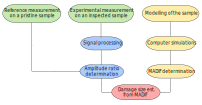
\includegraphics[width=1\linewidth]{Chapter_3/flowchart}
		\end{center}
	\caption{A flowchart representing the process for damage size estimation.}
	\label{fig:Flowchart}
\end{figure}

When the structure model is developed, several computer simulations for various damage sizes must be conducted to determine the \ac{madif}, a cornerstone of the dissertation. This function determines the severity of the \ac{hsc} damage based on the signal received by the sensor.
Several excitation signals and damage indices will be considered to select the best \ac{madif}.
The selection criterion will be the monotonicity and the function slope over the considered range of the damage size. Then, the damage magnitude is obtained from the \ac{madif} for the measured signal and normalised to the reference one.


 

\clearpage{}
\clearpage{}

\chapter[The Time-Domain Spectral Element Method Formulation]{The Time-Domain Spectral Element Method Formulation}
\label{ch:sem}





\section{The Spectral Element Method}
\label{sec:sem}



The general concept of the \ac{sem} is based on the idea of the \ac{fem}.
The similarity of both methods lies in the fact that the modelled domain is divided into non-overlapping finite elements, and external forces and arbitrary boundary conditions are imposed in the particular nodes.
The main difference between those methods is a choice of the shape function \( N=N(\xi )\), pictured in Fig.\ref{fig:shape}, which is interpolated by a Lagrange polynomial that passes through the element nodes.
The nodes are localized on the endpoint of an interval, \(\xi\in[-1,1]\), and the roots of the first derivative of Legendre polynomial P of degree \(p-1\):
\begin{eqnarray}
	(1-\xi^2)P'_{p-1}(\xi)=0.
	\label{eq:nodes}
\end{eqnarray}
The approximation of an integral over the elements is achieved according to \ac{gll} rule at points coinciding with the element nodes, 
and the weights \(w=w(\xi)\) calculated as:
\begin{eqnarray}
	{w(\xi)} = \frac{2}{p(p-1)(P_{p-1}(\xi))^2}.
	\label{eq:weights}
\end{eqnarray}

The shape functions and the weights for \ac{2d} or \ac{3d} elements are obtained by the Kronecker product of vectors of individual axes, denoted by \(\otimes\) as follows:
\begin{eqnarray}
	N(\xi,\eta) = N(\xi)\otimes N(\eta), & N(\xi,\eta,\zeta) = N(\xi)\otimes N(\eta)\otimes N(\zeta), \nonumber\\
	w(\xi,\eta) = w(\xi)\otimes w(\eta), & w(\xi,\eta,\zeta) = w(\xi)\otimes w(\eta)\otimes w(\zeta).
	\label{eq:3Dshape_weights}
\end{eqnarray}
\begin{figure}[H]
	\begin{center}
		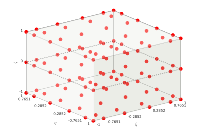
\includegraphics[width=1\linewidth]{Chapter_4/shape_function}
	\end{center}
	\caption{Shape functions for five order polynomial with Gaussa-Lobatto-Legendre nodes.}
	\label{fig:shape}
\end{figure}

The elementary equations of motion are defined as:
\begin{eqnarray}
	\label{eq:motion}
	\textbf{M} \ddot{\textbf{d}} + \textbf{D} \dot{\textbf{d}} + \textbf{K} \textbf{d} = \textbf{F}_{ext},
\end{eqnarray}
where \textbf{d} is the displacement vector; \textbf{M}, \textbf{D} and \textbf{K} are the structural mass, damping and stiffness matrices, respectively; \textbf{F}$_{ext}$ is the external forces vector; \((\dot{\ })=\frac{\partial}{\partial t}\). 
The construction of the structural matrices is similar to the classical approach in \ac{fem}.

The most significant advantage of this method is the fast convergence of the equation of motion.
It is achieved for six nodes per wavelength, while at least fifteen nodes are needed in the case of linear elements in classic \ac{fem}~\cite{wee2017simulating}.
Moreover, the mass matrix is diagonal when the \ac{gll} approach is used, and solid or classic, low-order displacement theory elements are involved.
 \section{2D Spectral Modelling}
\label{sec:2Dmodel}



According to the first-order shear deformation theory~\cite{reissner1945effect, mindlin1951influence}, the displacement field is expressed as:
\begin{eqnarray}
	\left \{ \begin{array}{c}
		\textbf{u}^e(\xi,\eta) \\
		\textbf{v}^e(\xi,\eta) \\
		\textbf{w}^e(\xi,\eta)
	\end{array} \right\} = 
	\left \{ \begin{array}{c}
		\textbf{u}_0^e(\xi,\eta) + z\boldsymbol{\varphi}_x^e(\xi,\eta)\\
		\textbf{v}_0^e(\xi,\eta) + z\boldsymbol{\varphi}_y^e(\xi,\eta)\\
		\textbf{w}_0^e(\xi,\eta) \\
	\end{array} \right\},
\end{eqnarray}
where \(\textbf{u}_0^e\), \(\textbf{v}_0^e\) and \(\textbf{w}_0^e\) are nodal displacements, \(\boldsymbol{\varphi}_x^e\), \(\boldsymbol{\varphi}_y^e\) are the rotations of the normal to the mid-plane with respect to the axes \textit{x} and \textit{y}, respectively. They are defined as:
\begin{eqnarray}
	\left \{\begin{array}{c}
		\textbf{u}_0^e(\xi,\eta) \\
		\textbf{v}_0^e(\xi,\eta) \\
		\textbf{w}_0^e(\xi,\eta) \\
		\boldsymbol{\varphi}_x^e(\xi,\eta) \\
		\boldsymbol{\varphi}_y^e(\xi,\eta)
	\end{array} \right\}
	= \textbf{N}^e(\xi,\eta)\widehat{\textbf{d}}^e
	= \sum_{n=1}^q\sum_{m=1}^p\textbf{N}_m^e(\xi)\textbf{N}_n^e(\eta)
	\left \{ \begin{array}{c}
		\widehat{\textbf{u}}_0^e \\
		\widehat{\textbf{v}}_0^e \\
		\widehat{\textbf{w}}_0^e \\
		\widehat{\boldsymbol{\varphi}}_x^e \\
		\widehat{\boldsymbol{\varphi}}_y^e
	\end{array} \right \},
\end{eqnarray}
where $\widehat{\textbf{d}}^e$ is a nodal displacements vector of the element $e$.

The nodal bending strain--displacement relations are given in the form:
\begin{eqnarray}
	\boldsymbol{\epsilon}_b^e =
	\textbf{B}_b^e\widehat{\textbf{d}}^e = 
	\left [
	\begin{array}{ccccc}
		\frac{\partial N^e}{\partial x} & 0 & 0 & 0 & 0\\
		0 & \frac{\partial N^e}{\partial y} & 0 & 0 & 0\\
		\frac{\partial N^e}{\partial y} & \frac{\partial N^e}{\partial x} & 0 & 0 & 0\\
		0 & 0 & 0 & -\frac{\partial N^e}{\partial x} & 0\\
		0 & 0 & 0 & 0 & -\frac{\partial N^e}{\partial y}\\
		0 & 0 & 0 & -\frac{\partial N^e}{\partial y} & -\frac{\partial N^e}{\partial x}
	\end{array} \right]
	\left \{ \begin{array}{c}
		\widehat{\textbf{u}}_0^e \\
		\widehat{\textbf{v}}_0^e \\
		\widehat{\textbf{w}}_0^e \\
		\widehat{\boldsymbol{\varphi}}_x^e \\
		\widehat{\boldsymbol{\varphi}}_y^e
	\end{array} \right\}.
\end{eqnarray}

The nodal shear strain--displacement relations are given in the form:
\begin{eqnarray}
	\boldsymbol{\epsilon}_s^e =
	\textbf{B}_s^e\widehat{\textbf{d}}^e = 
	\left [
	\begin{array}{ccccc}
		0 & 0 & \frac{\partial N^e}{\partial y} & -1 & 0\\
		0 & 0 & \frac{\partial N^e}{\partial y} & 0 & -1
	\end{array} \right]
	\left \{ \begin{array}{c}
		\widehat{\textbf{u}}_0^e \\
		\widehat{\textbf{v}}_0^e \\
		\widehat{\textbf{w}}_0^e \\
		\boldsymbol{\varphi}_x^e \\
		\boldsymbol{\varphi}_y^e
	\end{array} \right\}.
\end{eqnarray}

The mass and stiffness matrices for \ac{2d} elements are defined as:
\begin{eqnarray}
	\textbf{M}_{dd}^e & = &
	\left [
	\begin{array}{cc}
		\textbf{M}^e & 0\\
		0 & \textbf{J}^e
	\end{array}
	\right] =
	\int_{\Omega_e}\textbf{N}^T\rho
	\left [
	\begin{array}{ccccc}
		h & 0 & 0 & 0 & 0 \\
		& h & 0 & 0 & 0 \\
		&  & h & 0 & 0\\
		&  &  & \frac{h^3}{12} & 0\\
		Sym. &  &  &  & \frac{h^3}{12}
	\end{array} \right]
	\textbf{N} \diff\Omega_e,\\
	\textbf{K}_{dd}^e & = & \int_{\Omega_e}{\textbf{B}_b^e}^T
	\left[
	\begin{array}{cc}
		\textbf{A} & \textbf{B}\\
		\textbf{B} & \textbf{D}
	\end{array} \right]
	\textbf{B}_b^e \diff \Omega_e+\int_{\Omega_e}{\textbf{B}_s^e}^T\hat{\textbf{A}}\textbf{B}_s^e\diff \Omega_e,
\end{eqnarray}
where \(h=h_t+h_b\) is the element thickness, while \(h_{t(b)}\) is the distance between mid-plane and top(bottom) surface of the element, and \(\Omega_e\) is the element area:
\begin{eqnarray}
	\textbf{A} & = & \textbf{c}_{ij}\,(h_t-h_b),\qquad i,j=1,2,6\nonumber\\
	\textbf{B} & = & 1/2\, \textbf{c}_{ij}\,(h_t^2-h_b^2),\qquad i,j=1,2,6\nonumber\\
	\textbf{D} & = & 1/3\, \textbf{c}_{ij}\,(h_t^3-h_b^3),\qquad i,j=1,2,6\nonumber\\
	\hat{\textbf{A}} & = & 5/4\, \textbf{c}_{ij}\,\left[h_t-h_b-4/3\left(h_t^3-h_b^3\right)/h^2\right],\qquad i,j=4,5.
\end{eqnarray}
 \section{3D Spectral Modelling}
\label{sec:3Dmodel}

The displacement vector of the \ac{3d} element is composed of three translational displacements defined as:
\begin{eqnarray}
	\left \{ \begin{array}{c}
		\textbf{u}^e(\xi,\eta,\zeta) \\
		\textbf{v}^e(\xi,\eta,\zeta) \\
		\textbf{w}^e(\xi,\eta,\zeta)
	\end{array} \right\}
	= \textbf{N}^e(\xi,\eta, \zeta)\widehat{\textbf{d}}^e
	= \sum_{l=1}^r\sum_{n=1}^q\sum_{m=1}^p\textbf{N}_m^e(\xi)\textbf{N}_n^e(\eta)\textbf{N}_l^e(\zeta)
	\left \{ \begin{array}{c}
		\widehat{\textbf{u}}^e(\xi_m,\eta_n,\zeta_l) \\
		\widehat{\textbf{v}}^e(\xi_m,\eta_n,\zeta_l) \\
		\widehat{\textbf{w}}^e(\xi_m,\eta_n,\zeta_l)
	\end{array} \right\},
	\label{eq:3D_displ}
\end{eqnarray}
where \(\widehat{\textbf{u}}^e\), \(\widehat{\textbf{v}}^e\) and 
\(\widehat{\textbf{w}}^e\) are displacements of the element nodes in \(\xi,\eta\) and \(\zeta\) direction.

The nodal strain--displacement relations are given as \cite{kudela20093d}:
\begin{eqnarray}
	\boldsymbol{\epsilon}^e=\textbf{B}_{d}^e\widehat{\textbf{d}}^e=
	\left [
	\begin{array}{ccc}
		\frac{\partial N^e}{\partial x} & 0 & 0\\
		0 & \frac{\partial N^e}{\partial y} & 0\\
		0 & 0 & \frac{\partial N^e}{\partial z}\\
		0 & \frac{\partial N^e}{\partial z} & \frac{\partial N^e}{\partial y}\\
		\frac{\partial N^e}{\partial z} & 0 & \frac{\partial N^e}{\partial x}\\
		\frac{\partial N^e}{\partial y} & \frac{\partial N^e}{\partial x} & 0
	\end{array} \right]
	\left \{ \begin{array}{c}
		\widehat{\textbf{u}}^e \\
		\widehat{\textbf{v}}^e \\
		\widehat{\textbf{w}}^e
	\end{array} \right\}.
\end{eqnarray}
The formulae of the structural matrices for 3D elements are:
\begin{eqnarray}
	\textbf{M}_{dd}^e & = & \int_{V_e}\textbf{N}^T\rho \textbf{N} \diff V_e,\\
	\textbf{K}_{dd}^e & = & \int_{V_e}{\textbf{B}_d^e}^T\textbf{C}\textbf{B}_d^e \diff V_e,
\end{eqnarray}
where \textbf{C} is the stiffness tensor, \(\rho\) is mass density, and \(V_e\) is the element volume. \section{\ac{pzt} Modelling}
\label{sec:PZTmodel}

The electromechanical coupling is governed by the linear constitutive equation of piezoelectric material according to~\cite{giurgiutiu2009micromechatronics, rekatsinas2017cubic}, and this is defined as:
\begin{eqnarray}
	\left [ 
	\begin {array}{c}
	\boldsymbol{\sigma}\\
	\textbf{D}
\end{array}\right ]=
\left [ 
\begin{array}{cc}
	\textbf{c}^E & -\textbf{e}^T \\
	\textbf{e} & \epsilon^S 
\end{array} \right ]
\left[ 
\begin{array}{c}
	\textbf{S}\\
	\textbf{E} 
\end{array} \right ],
\label{eq:elecmechcoupling}
\end{eqnarray}
where \(\boldsymbol{\sigma}\) and \(\textbf{S}\) are the stress and strain components, respectively, \(\textbf{c}^E\) is the stiffness coefficient matrix measured at zero electric field, \textbf{e} is the piezoelectric coupling tensor,  \(\boldsymbol{\epsilon}^S\) is the electric permittivity, and \textbf{E} and \textbf{D} are the electric field and electric displacement measured at zero strain.
The superscript T denotes a transpose matrix.
The electric field is defined as:
\begin{eqnarray}
\textbf{E}^e=-\textbf{B}_\phi^e \widehat{\boldsymbol{\phi}}^e = \left[ \begin{array}{c}
	\frac{\partial N^e}{\partial \xi}\\
	\frac{\partial N^e}{\partial \eta}\\
	\frac{\partial N^e}{\partial \zeta}
\end{array} \right] \widehat{\boldsymbol{\phi}}^e.
\end{eqnarray}
where \(\widehat{\boldsymbol{\phi}}^e\) is a nodal voltage of the transducer. The \ac{sem} formulation of the governing equation \ref{eq:elecmechcoupling} is defined as:
\begin{eqnarray}
	\left [\begin{array}{cc}
		\textbf{M}_{dd} & \textbf{0}\\
		\textbf{0} & \textbf{0}
	\end{array}\right]
	\left \{\begin{array}{c}
		\widehat{\ddot{\textbf{d}}} \\
		\textbf{0}
	\end{array}\right \} +
	\left [\begin{array}{cc}
		\textbf{K}_{dd} & \textbf{K}_{d \phi}\\
		\textbf{K}_{d \phi}^T & \textbf{K}_{\phi \phi}
	\end{array}\right]
	\left \{\begin{array}{c}
		\widehat{\textbf{d}} \\
		\widehat{\boldsymbol{\phi}}
	\end{array}\right \}  = 
	\left \{\begin{array}{c}
		\textbf{0}\\
		\widehat{\textbf{Q}}
	\end{array}\right \},
	\label{eq:pzt_sem}
\end{eqnarray}
where \(\textbf{Q}\) is the nodal charge vector.
The mass and stiffness matrices are defined according to \ac{3d} model from section \ref{sec:3Dmodel}.
The piezoelectric coupling matrix \(\textbf{K}_{\phi \phi}^e\) and the dielectric permittivity matrix \(\textbf{K}_{d \phi}^e\) are defined as:
\begin{eqnarray}
	\textbf{K}_{d\phi}^e & = & \int_{V_e}{\textbf{B}_d^e}^T\textbf{e}^T \textbf{B}_{\phi}^e \diff V_e,\\
	\textbf{K}_{\phi \phi}^e & = & -\int_{V_e}{\textbf{B}_{\phi}^e}^T 
	{\textbf{\(\epsilon\)}^S}^T \textbf{B}_{\phi}^e \diff V_e.
\end{eqnarray}

If a vector \(\textbf{b}\) contains an order list of boundary nodes (electrodes) and a vector \(\textbf{a}\) contains an order lists of active nodes (remains nodes) of the \ac{pzt}, the electrical potential vector and the charge vector can be rewritten as:
\begin{eqnarray}
	\widehat{\boldsymbol{\phi}} = \left \{\begin{array}{cc}
		\widehat{\boldsymbol{\phi}}(\textbf{b}) &
		\widehat{\boldsymbol{\phi}}(\textbf{a})
	\end{array}\right \}^T,\\
	\widehat{\textbf{Q}} = \left \{\begin{array}{cc}
		\widehat{\textbf{Q}}(\textbf{b}) & \textbf{0}
	\end{array}\right \}^T.
	\label{eq:phi_Q}
\end{eqnarray}
Then, piezoelectric part of Equation~(\ref{eq:pzt_sem}) is expressed as:
\begin{eqnarray}
	\left [\begin{array}{cc}
		\textbf{K}_{d \phi}(:,\textbf{b}) &
		\textbf{K}_{d \phi}(:,\textbf{a})
	\end{array}\right]^T
	\widehat{\textbf{d}} +
	\left [\begin{array}{cc}
		\textbf{K}_{\phi \phi}(\textbf{b},\textbf{b}) & \textbf{K}_{\phi \phi}(\textbf{b},\textbf{a})\\
		\textbf{K}_{\phi \phi}(\textbf{a},\textbf{b}) & \textbf{K}_{\phi \phi}(\textbf{a},\textbf{a})
	\end{array}\right]
	\left \{\begin{array}{c}
		\widehat{\boldsymbol{\phi}}(\textbf{b}) \\
		\widehat{\boldsymbol{\phi}}(\textbf{a})
	\end{array}\right \} = 
	\left \{\begin{array}{c}
		\widehat{\textbf{Q}}(\textbf{b}) \\
		\textbf{0}
	\end{array}\right \},
	\label{eq:pztboundary}
\end{eqnarray}
where the notation \(\textbf{K}(\textbf{r},\textbf{c})\) uses vectors \(\textbf{r}\) and \(\textbf{c}\) to extract rows and columns from the matrix \(\textbf{K}\), respectively, and \((:)\) means all rows or columns of \(\textbf{K}\).
The electrical potential of the free nodes can be extracted from Equation~(\ref{eq:pztboundary}):
\begin{eqnarray}
	\widehat{\boldsymbol{\phi}}(\textbf{a}) = -\textbf{K}_{\phi\phi}^{-1}(\textbf{a},\textbf{a})\left[\textbf{K}_{\phi d}(\textbf{a},:) \widehat{\textbf{d}} + \textbf{K}_{\phi\phi}(\textbf{a},\textbf{b})\widehat{\boldsymbol{\phi}}(\textbf{b}) \right].
	\label{eq:freePotetial}
\end{eqnarray}
If the \ac{pzt} acts as an actuator, the electrical potential of the electrode nodes has the values of the applied signal.
As one of the electrodes is grounded, the potential is zero.
Therefore, the potential vector can be written as:
\begin{eqnarray}
	\widehat{\boldsymbol{\phi}}(\textbf{b}) = \left \{\begin{array}{cc}
		\widehat{\boldsymbol{\phi}}(\textbf{b}_v) &
		\widehat{\boldsymbol{\phi}}(\textbf{b}_g)
	\end{array}\right \}^T=\left \{\begin{array}{cc}
	\textbf{V}(t) & \textbf{0}
	\end{array}\right \}^T,
	\label{eq:phi_V}
\end{eqnarray}
where \(\textbf{b}_v\) is a list of nodes of the applied electrode and \(\textbf{b}_g\) is a list of nodes of the grounded electrode.
Substituting Equation \ref{eq:phi_V} into Equations \ref{eq:freePotetial} and \ref{eq:pztboundary} induced stiffness of the actuator is obtained:
\begin{eqnarray}
	\textbf{K}_{a}=-\textbf{K}_{d\phi}(:,\textbf{a})\,\textbf{K}_{\phi \phi}^{-1}(\textbf{a},\textbf{a})\,\textbf{K}_{\phi \phi} (\textbf{a},\textbf{b}).
\end{eqnarray}
Hence, the equivalent mechanical force vector of the applied voltage of the piezoelectric actuator equals:
\begin{eqnarray}
	\widehat{\textbf{f}}_{act}=-\textbf{K}_{a}\,\widehat{\boldsymbol{\phi}}(\textbf{b})
	\label{eq:f_act}
\end{eqnarray}

In the case of the open circuit sensor one electrode is grounded so the electric potential of the free nodes becomes as:
\begin{eqnarray}
	\widehat{\boldsymbol{\phi}}(\textbf{a}) = -\textbf{K}_{\phi\phi}^{-1}(\textbf{a},\textbf{a})\,\textbf{K}_{\phi d}(\textbf{a},:)\,\widehat{\textbf{d}}.
	\label{eq:sensorPotetial}
\end{eqnarray}
The induced stiffness of the sensor can be written as:
\begin{eqnarray} \textbf{K}_s=\textbf{K}_{d \phi}(:,\textbf{a})\,\textbf{K}_{\phi \phi}^{-1} (\textbf{a},\textbf{a})\,\textbf{K}_{\phi d}(\textbf{a},:).
\end{eqnarray}
To obtain the sensor response nodal electric potential must be integrated over the electrode surface as follow:
\begin{eqnarray}
	\boldsymbol{\phi}(t) = \int_{\Omega_s}\widehat{\phi} \diff\Omega_s.
	\label{eq:sensorResponse}
\end{eqnarray} \section{Structural Damping}
\label{sec:damping}

Propagating waves in the structure attenuate due to many factors, including geometric spreading, material damping, and dissipation into the adjacent domain.
This study adopted the Rayleigh damping model for the \ac{cfrp} skin and adhesive layer, while the damping for the aluminium core and \ac{pzt} was neglected.
Rayleigh damping model is defined as \cite{wandowski2017guided}
\begin{eqnarray}
	\textbf{D}_{dd}^e = \alpha_M \textbf{M}_{dd}^e + \beta_K \textbf{K}_{dd}^e.
	\label{eq:damping}
\end{eqnarray}
where \(\alpha_M\) and \(\beta_K\) are the mass- and stiffness- proportionality coefficients. However, \(\beta_K\) is equal to zero to ensure that matrix \(\textbf{D}_{dd}\) remains diagonal. \section{Displacements Coupling at the Interface of Substructures}
\label{sec:interface}



The present model of the sandwich panel consists of \ac{2d} and \ac{3d} elements. 
Moreover, there are non-matching grids between two adjacent substructures. 
These involve connecting them by imposing the compatibility of the displacements at the interface, see Fig.~\ref{fig:interface}.
This type of connection is implemented through the interface elements based on Lagrange multipliers, which are interpreted as forces responsible for determining the appropriate displacements of nodes.
The coupling can be expressed as:
\begin{eqnarray}
	\left\{\begin{array}{c}
		\textbf{u}\\
		\textbf{v}\\
		\textbf{w}
	\end{array}\right\}_{s_{i1}}^{\Gamma^i}-
	\left\{\begin{array}{c}
		\textbf{u}\\
		\textbf{v}\\
		\textbf{w}
	\end{array}\right\}_{s_{i2}}^{\Gamma^i}=
	\left\{\begin{array}{c}
		\textbf{0}\\
		\textbf{0}\\
		\textbf{0}
	\end{array}\right\},
	\label{eq:coupling}
\end{eqnarray}
\begin{figure}
	\begin{center}
		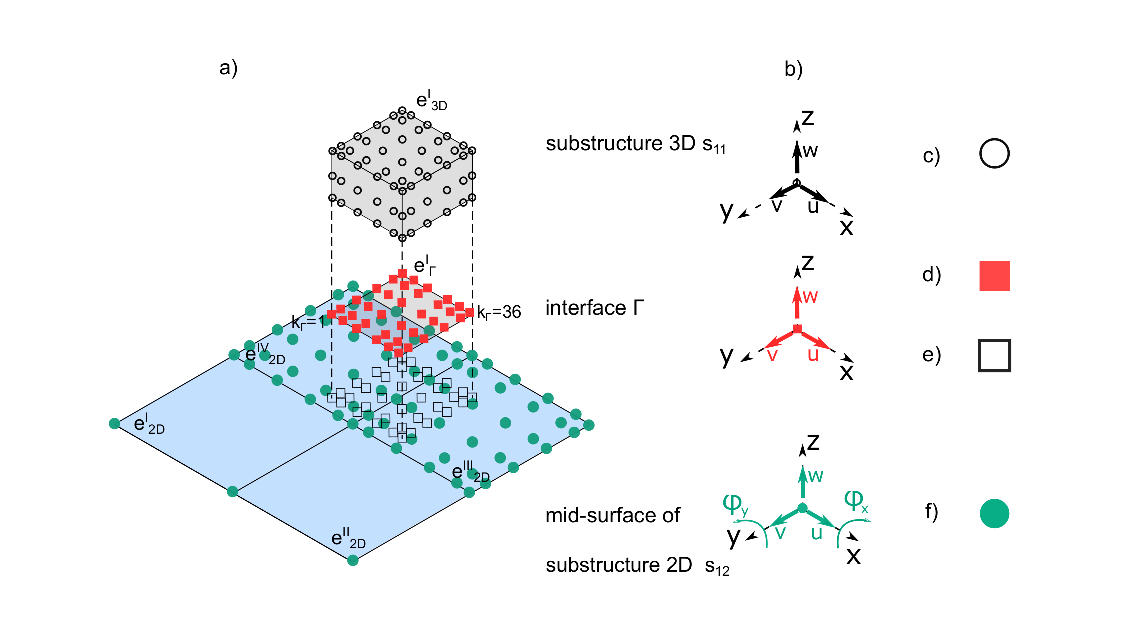
\includegraphics[scale=0.8]{Chapter_4/interface_2D3D}
	\end{center}
	\caption{Non-matching interface setup: a) interface coupling, b) degrees-of-freedom of the interface and the substructures.}
	\label{fig:interface}
\end{figure}
where \(s_{i1}\) and \(s_{i2}\) are substructures connected by the interface \(\Gamma^i\). For the whole structure, the Eq.~(\ref{eq:coupling}) can be written in the matrix form:
\begin{eqnarray}
	\textbf{G}\textbf{d}=\textbf{0},
	\label{eq:cond_disp}
\end{eqnarray}
where \textbf{G} is the coupling matrix which contains the equations to interpolate the substructures displacements at the interfaces, and \(\textbf{d}\) is a global displacement field for \(nS\) number of substructures, composed as:
\begin{eqnarray}
	\textbf{d} = \left\{\begin{array}{cccc}
		\textbf{d}_1, & \textbf{d}_2, &\ldots, & \textbf{d}_{nS}
	\end{array}\right\}^T.
	\label{eq:displacements}
\end{eqnarray}

General formulation of the matrix \textbf{G} is presented in Algorithm \ref{alg:G_matrix}.

\begin{algorithm}[H]
	\SetAlgoLined
	\KwResult{coupling matrix \textbf{G}}
	\For{i = 1 \KwTo 2}{
		create \(n^{\Gamma}\times n^{s_i}\) null matrix 
		\(\mathbf{G}_i\),\\
		\For{j = 1 \KwTo \(n^{\Gamma}\)} {
			find \(ownerElement^j_i\) in the structure \(s_i\) 
			containing interface node \(j\) with global coordinates vector: 
			\(X_p=(x^j_p,y^j_p)\)\;
			assign vector \(X_e=(x_e,y_e)\) of coordinates of all nodes in 
			\(ownerElement^j_i\)\;
			assign initial coordinates 
			\(X_{\kappa}=(x^j_{\kappa},y^j_{\kappa})\) to the nearest node in
			\(ownerElement^j_i\) to node \(j\)\;
			transform global coordinates \(X_{\kappa}\) to a local coordinate system \(\xi_{\kappa}=\xi(X_{\kappa});\quad 
			\eta_{\kappa}=\eta(X_{\kappa})\)\;
			\While{\(\left|X_p-X_{\kappa}\right|>tol\)}{
				\(\xi_{\kappa+1}=\xi_{\kappa}+(J^{-1}_{\kappa})_{11}.*(x^j_p-x_{\kappa}^j)
				+(J^{-1}_{\kappa})_{12}.*(y^j_p-y_{\kappa}^j)\)\;
				\(\eta_{\kappa+1}=\eta_{\kappa}+(J^{-1}_{\kappa})_{21}.*(x^j_p-x_{\kappa}^j)
				+(J^{-1}_{\kappa})_{22}.*(y^j_p-y_{\kappa}^j)\)\;
				\(X_{\kappa}=N_{\kappa+1}X_e\)\;
			}
			\(\mathbf{G}_i(j,n^{X_e})=N_{\kappa+1}\)\;
		}
		\uIf{\(s_i\) is 3D} {
			\(\mathbf{G}_i=\left[\begin{array}{ccc}
				\mathbf{G}_i & \mathbf{0} & \mathbf{0}\\
				\mathbf{0} & \mathbf{G}_i & \mathbf{0}\\
				\mathbf{0} & \mathbf{0} & \mathbf{G}_i
			\end{array} \right]
			\)\;
		}
		\ElseIf{\(s_i\) is 2D} {
			\(\mathbf{G}_i=\left[\begin{array}{ccccc}
				\mathbf{G}_i & \mathbf{0} & \mathbf{0} & 
				\frac{h_i}{2}\mathbf{G}_i & \mathbf{0}\\
				\mathbf{0} & \mathbf{G}_i & \mathbf{0} & \mathbf{0} & 
				\frac{h_i}{2}\mathbf{G}_i\\
				\mathbf{0} & \mathbf{0} & \mathbf{G}_i & \mathbf{0} & 
				\mathbf{0}
			\end{array} \right]\)\;
		}
	}
	\(\mathbf{G}=\left[\begin{array}{cc}
		\mathbf{G}_1 & \mathbf{G}_2
	\end{array} \right].\)
	\caption{Interface coupling matrix formulation}
	\label{alg:G_matrix}
\end{algorithm}
where \(s_i\) is the structure to, \(n^{\Gamma}\) and \(n^{s_i}\) are numbers of nodes of the interface, respectively; \(J_{\kappa}\) is the Jacobian evaluated at \((\xi_{\kappa},\eta_{\kappa})\) and \(N_{\kappa+1}\) is the shape function evaluated at \((\xi_{\kappa+1},\eta_{\kappa+1})\), \(n^{X_e}\) is the vector of global order numbers of all nodes in the \(ownerElements^j_i\), \(h_i\) is a thickness of the structure \(s_i\) and \(tol\) is a termination criterion for iterations.

The main task of the algorithm is to calculate shape functions for each adjacent substructures at the points \(X_p=(x_p^k,y_p^k)\), which are projections of the interface nodes onto these substructures.
The shape function can be calculated after finding an owner element and local coordinates of the points.
Owner element is a spectral element in the domain of the substructure \(s_{ij}\) which contains interface node, for example, interface node \(k_\Gamma=36\) (see~Fig.~\ref{fig:interface}a)) is located in the element \(e^{I}_{3D}\) and \(e^{III}_{2D}\) for the substructures \(s_{11}\) and \(s_{12}\), respectively.
It can be found within two ways: using Matlab's built-in function \verb+inpolygon+ or more efficient procedure proposed by Silva et al. \cite{silva2009exact} which was used in the current implementation.
The transformation from global to local coordinates was realized by the iterative method presented in the work of Li et al.~\cite{li2014efficient}.
The computational effectiveness of Algorithm~\ref{alg:G_matrix} can be easily improved if certain precautions are taken.
Firstly, the mesh of the interface has to be based on the mesh from one of the substructures \(s_{i1}\), \(s_{i2}\), which may be referred to as a slave.
So, the shape function takes only the values of one and zeros.
Moreover, the code can be implemented in vectorized form rather than using a for-loops. \section{The Time Integration}
\label{sec:time}

Similar to the \ac{fem}, the time solution of the governing equation can be realized implicitly, e.g., by the the Crank-Nicolson
scheme, or explicitly, e.g., by the central difference method \cite{bathe2006finite}.
The first method for specific parameters is an absolutely stable algorithm, i.e., independent of the time step.
In contrast, a much smaller time step in the explicit method than that required by the Nyquist-Shannon sampling theorem must be taken.
The critical value of time increment (\(\Delta t_{cr}\)) depends on the mesh size and the wave mode velocity.
The most significant advantage of this method is that only the sum of the mass and damping matrices needs to be inverted, which is trivial in the presented scheme because both matrices are diagonal.

Considering piezoelectric coupling \ref{eq:elecmechcoupling} and the displacement interface \ref{eq:cond_disp} the global equation of motion is expressed as:

\begin{eqnarray}
	\label{eq:motion_coupling}
	\textbf{M}_{dd} \widehat{\ddot{\textbf{d}}} +
	\textbf{D}_{dd}	\widehat{\dot{\textbf{d}}} +
	\left [\begin{array}{ccc}
		\textbf{K}_{dd}&\textbf{K}_{d\phi}&\textbf{G}^T\\
		\textbf{K}_{d\phi}^T&\textbf{K}_{\phi \phi}&\textbf{0}\\
		\textbf{G}&\textbf{0}&\textbf{0}
	\end{array}\right]
	\left \{\begin{array}{c}
		\widehat{\textbf{d}}\\
		\widehat{\boldsymbol{\phi}}\\
		\widehat{\boldsymbol{\lambda}}
	\end{array}\right\} =
	\left \{\begin{array}{c}
		\widehat{\textbf{f}}_{ext} \\
		\widehat{\textbf{Q}}\\
		\textbf{0}
	\end{array}\right \},
\end{eqnarray}
\(\widehat{\boldsymbol{\lambda}}\) is the nodal Lagrange multipliers vector.
Substituting Equations~(\ref{eq:pztboundary}) and (\ref{eq:freePotetial}) into Equation~(\ref{eq:motion_coupling}), the equation of motion can be rearranged into the form:
\begin{eqnarray}
	\textbf{M}_{dd} \widehat{\ddot{\textbf{d}}} + \textbf{D}_{dd} \widehat{\dot{\textbf{d}}} + (\textbf{K}_{dd}-\textbf{K}_{s}) \widehat{\textbf{d}}  = \widehat{\textbf{f}}_{ext} + \widehat{\textbf{f}}_{a} - \textbf{G}^T \widehat{\boldsymbol{\lambda}}.
	\label{eq:motionD}
\end{eqnarray}
In the scheme of central difference method, the velocity and acceleration at a certain time t is given by:
\begin{eqnarray}
	\label{eq:v}
	\dot{\textbf{d}}_{t} = \frac{\textbf{d}_{t+\Delta t} - \textbf{d}_{t-\Delta t}}{2\Delta t},\\
	\label{eq:a}
	\ddot{\textbf{d}}_{t} = \frac{\textbf{d}_{t+\Delta t} - 2\textbf{d}_{t} + \textbf{d}_{t-\Delta t}}{\Delta t^2},
\end{eqnarray}
where \(\Delta t\) is the time increment, \(\textbf{d}_{t}\), \(\textbf{d}_{t-\Delta t}\) and \(\textbf{d}_{t+\Delta t}\) are the nodal displacements vectors in time t, one step back and forward, respectively. 
Thus, substituting Equations \ref{eq:v} and \ref{eq:a} into Equation~(\ref{eq:motionD}) and after some modification global equation of motion can be expressed as:
\begin{equation}
	\begin{array}{c}
		\left(\frac{1}{\Delta t^2}\textbf{M}_{dd}+\frac{1}{2\Delta t}\textbf{D}_{dd} \right)\widehat{\textbf{d}}_{t+\Delta t}=
		\widehat{\textbf{f}}_{ext} + \widehat{\textbf{f}}_{a} - \left( \textbf{K}_{dd}-\textbf{K}_s\right)\widehat{\textbf{d}}_t+\\
		+\frac{2}{\Delta t^2}\textbf{M}_{dd}\widehat{\textbf{d}}_t-\left(\frac{1}{\Delta t^2}\textbf{M}_{dd}-\frac{1}{2\Delta t}\textbf{D}_{dd}\right)\widehat{\textbf{d}}_{t-\Delta t}-\textbf{G}^T\widehat{\boldsymbol{\lambda}}_t.
	\end{array}
	\label{eq:cdm}
\end{equation}

The vector of Lagrange multipliers \(\widehat{\boldsymbol{\lambda}}_t\) can be extracted from Equation~(\ref{eq:cdm}) by imposing the constrain (\ref{eq:cond_disp}): 
\begin{eqnarray}
	\widehat{\boldsymbol{\lambda}}_t = {\left(\textbf{G}\textbf{L}_+^{-1}\textbf{G}^T \right)}^{-1}\textbf{G}\textbf{L}_+^{-1} \Bigg[ \widehat{\textbf{f}}_{ext} + \widehat{\textbf{f}}_{a} + \left.\left(\frac{2}{\Delta t^2}\textbf{M}_{dd}-\textbf{K}_{dd}+\textbf{K}_s\right)\widehat{\textbf{d}}_t -\textbf{L}_-\widehat{\textbf{d}}_{t-\Delta t} \right],
	\label{eq:lambda}
\end{eqnarray}
where \(\textbf{L}_{\pm}=\frac{1}{\Delta t^2}\textbf{M}_{dd}\pm\frac{1}{2\Delta t}\textbf{C}_{dd}\).
The implementation of the central difference method is presented in Algorithm~\ref{alg:cdm}.
The implementation concerns the excitation and reception of the wave by a pair of \acp{pzt}.

\begin{algorithm}[H]
	\SetAlgoLined
	\KwResult{nodal displacement vector \(\widehat\textbf{d}_{t+\Delta t}\) and sensore response \(\boldsymbol{\phi}_{t+\Delta t}\)}
	initialise  \(\widehat{\textbf{d}}_0\), \(\widehat{\dot{\textbf{d}}}_0\), \(\widehat{\boldsymbol{\lambda}}_0\) and \(\boldsymbol{\phi}_{0}\)\\
	calculate \(\widehat{\ddot{\textbf{d}}}_0\) from Equation~\ref{eq:motionD},\\
	select time step \(\Delta t<=\Delta t_{cr}\),\\
	extract \(\widehat{\textbf{d}}_{0-\Delta t}\) from Equations \ref{eq:v} and \ref{eq:a},\\
	\For{each time step}{
	calculate actuator forces \(\widehat{\textbf{f}}_a\) by Equation~\ref{eq:f_act},\\
	calculate internal forces \(\widehat{\textbf{f}}_{int}=\left(\textbf{K}_{dd}-\textbf{K}_{s}\right)\,\widehat{\textbf{d}}_t\),\\
	calculate Lagrange multipliers \(\widehat{\boldsymbol{\lambda}}\) by Equation~\ref{eq:lambda},\\
	calculate following step displacement \(\widehat{\textbf{d}}_{t+\Delta t}\) solving equation of motion \ref{eq:cdm},\\
	calculate sensore response \(\boldsymbol{\phi}_{t+\Delta t}\) by Equation \ref{eq:sensorResponse}.
	}
	\caption{Central difference method implementation}
	\label{alg:cdm}
\end{algorithm}

 \section{Parallel Implementation of the Internal Force Vector Calculation}
\label{sec:gpu}


The most time-consuming operation in the equation (\ref{eq:motion}) is calculating the internal force vector \(\textbf{f}_{int}=\left(\textbf{K}_{dd}-\textbf{K}_{s}\right)\widehat{\textbf{d}}_{t}\), as the stiffness matrix \(\textbf{K}_{dd}\) occupies a large amount of memory.
Instead of allocating the full matrix \(\textbf{K}_{dd}\), Kudela proposed a parallelized computation of the internal force vector \cite{kudela2016parallel}.
In the pre-processing, the natural derivatives matrix, the vector of inverted components of the Jacobian matrix, and the integration weights multiplied by the Jacobian determinant is rearranged from global to the local form:
\begin{eqnarray}
	\label{eq:isoparametric}
	\textbf{N}^P_{,\xi} & = & \left[ \begin{array}{cccc}
		\textbf{N}^{e=1}_{,\xi} & \textbf{0} & \ldots & \textbf{0}\\
		\textbf{0} & \textbf{N}^{e=2}_{,\xi} & \ldots & \textbf{0}\\
		\vdots & \vdots &  \ddots & \vdots\\
		\textbf{0} & \textbf{0} & \ldots & \textbf{N}^{e=n}_{,\xi}
	\end{array}\right],\\
	\label{eq:jacob}
	\left(\textbf{J}^P\right)^{ij}_{inv} & = & \left\{ \begin{array}{c}
		\left(\textbf{J}^{e=1}\right)^{ij}_{inv}\\
		\left(\textbf{J}^{e=2}\right)^{ij}_{inv}\\
		\vdots\\
		\left(\textbf{J}^{e=n}\right)^{ij}_{inv} \end{array}\right\},\\
	\label{eq:intWeights}
	\textbf{w}^P & = & \left\{ \begin{array}{c}
		\textbf{w}^{e=1}\\
		\textbf{w}^{e=2}\\
		\vdots\\
		\textbf{w}^{e=n} \end{array}\right\} \circ
	\left\{ \begin{array}{c}
		det(\textbf{J})^{e=1}\\
		det(\textbf{J})^{e=2}\\
		\vdots\\
		det(\textbf{J})^{e=n} \end{array}\right\},
\end{eqnarray}
where $n$ is the spectral elements number in modeled domain; \textbf{J} is the Jacobian matrix; $i,j=1\ldots3$; and $\circ$ denotes element-wise multiplication.
The $\textbf{N}^P_{,\xi}$ is a block-diagonal sparse matrix, and the equality of $\textbf{N}^1_{,\xi}=\textbf{N}^2_{,\xi}=\ldots=\textbf{N}^n_{,\xi}$ holds if the same order of interpolation shape function is used for the all elements.
Besides, a vector of local node indices $\textbf{I}_L$ and corresponding global node indices $\textbf{I}_G$ must be defined in the preprocessing process.

Adjacent elements in the mesh share nodes, so one node in the global system can correspond to several nodes in the local system. Since independent operations on vectors are necessary for parallel computation on \ac{gpu}, $I_{G}$ must be rearranged to separate all duplicated nodes. Therefore, the matrix $I_{G}$ is created in which no column has repeated indices of the nodes. Then, the corresponding local map $I_{L}$ must also be created. For the rearrangement algorithm presented in \cite{kudela2016parallel} was used.

The following computational operations are performed during the time integration algorithm. Firstly, the global vector of nodal displacements is transferred to the element nodes displacements such as:

\begin{eqnarray}
	\widehat{\textbf{d}}_t^P = \left\{ \begin{array}{c}
		\widehat{\textbf{d}}_t^{e=1}\\
		\widehat{\textbf{d}}_t^{e=2}\\
		\vdots\\
		\widehat{\textbf{d}}_t^{e=n} \end{array}\right\}.
\end{eqnarray}
Next, the strain and stress vectors are calculated as:
\begin{eqnarray}
	\label{eq:strain}
	\boldsymbol{\epsilon}=\left[\boldsymbol{\epsilon}_{xx},\ \boldsymbol{\epsilon}_{yy},\ \boldsymbol{\epsilon}_{zz},\ \boldsymbol{\gamma}_{yz},\ \boldsymbol{\gamma}_{xz},\ \boldsymbol{\gamma}_{xy}\ \right]^T&=&\textbf{B}^e\widehat{\textbf{d}}^e,\\
	\label{eq:stress}
	\boldsymbol{\sigma}=\left[\boldsymbol{\sigma}_{xx},\ \boldsymbol{\sigma}_{yy},\ \boldsymbol{\sigma}_{zz},\ \boldsymbol{\tau}_{yz},\ \boldsymbol{\tau}_{xz},\ \boldsymbol{\tau}_{xy},\ \right]^T&=&\textbf{C}\boldsymbol{\epsilon}.
\end{eqnarray}
The formulation of equation~\ref{eq:strain} and equation~\ref{eq:stress} for 3D and first-order shear deformation model can be found in \cite{kudela2016parallel} and \cite{kudela2020parallel}, respectively.
Then, the internal forces vector is calculated as:
\begin{eqnarray}
	\label{eq:forces}
	\textbf{F}^P_{int}=\left[\textbf{F}^P_1,\ \textbf{F}^P_2,\ \ldots\ \textbf{F}^P_{n} \right]^T={\textbf{B}^e}^T\boldsymbol{\sigma},
\end{eqnarray}
where $n$ is the nodal degree of freedom.
It should be mentioned that \(\boldsymbol{\epsilon}\), \(\boldsymbol{\sigma}\) and \(\textbf{F}^P_{int}\) components are calculated separately, with the appropriate order of performing the element-wise multiplication of the particular vectors.
This approach is essential in order to keep the calculations matrix-free.

Finally, the assembly of internal forces vector is performed using the \(\textbf{I}_G\) and \(\textbf{I}_L\) as follows:

\begin{eqnarray}
	\label{eq:Fint}
	{\left(\textbf{F}_{int}\right)}^t_{\textbf{I}^m_G} = {\left(\textbf{F}_{int}\right)}^t_{\textbf{I}^m_G} + {\left(\textbf{F}^P_{int}\right)}^t_{\textbf{I}^m_L},\quad for\ m=1\ldots col 
\end{eqnarray}
where \(col\) is the column number of \(\textbf{I}_G\).

In the dissertation, some improvements have been implemented to the above algorithm to make it more computationally efficient.
Instead of calculating the internal forces vector in the for loop like in equation~(\ref{eq:Fint}), it is recommended to assign all local forces into the matrix as:
\begin{eqnarray}
	\label{eq:Fmatrix}
	{\left(\textbf{F}_{int}\right)}^i_{\textbf{I}_G} ={\left(\textbf{F}^P_{int}\right)}^i_{\textbf{I}_L}
\end{eqnarray}
and then return the column vector containing the sum of each row of matrix \({\left(\textbf{F}^P_{int}\right)}^i_{\textbf{I}_L}\).
For example in Matlab, it can be done by built-in function \verb|sum| as:
\begin{eqnarray}
	\label{eq:Fsum}
	{\left(\textbf{F}_{int}\right)}^i = \verb|sum| \left({\left(\textbf{F}^P_{int}\right)}^i_{\textbf{I}_L},2\right);
\end{eqnarray}
Fixed number of columns in equation~(\ref{eq:Fint}) was proposed in \cite{kudela2016parallel}. In the current approach the number of columns is chosen adaptively according to the given mesh. It should be chosen as the smallest divisor of the number of nodes in an element but not less than the maximum number of common elements for a node. In this way, less serial operations are performed and \ac{gpu} resources are better utilized.

Further code modifications included storage scheme. Instead of storing in memory both isoparametric derivatives equation~(\ref{eq:isoparametric}) and inverted components of Jacobian matrix shown in equation~(\ref{eq:jacob}), it is recommended to calculate derivatives in global coordinates system as:
\begin{eqnarray}
	\textbf{N}^P_{,X} = \textbf{J}^{-1}\,\textbf{N}^P_{\xi} 
\end{eqnarray}
Also, a multiplication of elastic constants \(\textbf{C}\) with integration weights defined in equation (\ref{eq:intWeights}) can be performed in preprocessing stage before main loop through integration time steps.
 \section{Transformation of the Core Elements}
\label{sec:transformation}

All core elements are rotated relative to both skins, and thus it is necessary to transform the degrees of freedom from the local coordinate system of the core to the global coordinate system.
For this purpose, an additional sixth \ac{dof} is incorporated, i.e., rotation with respect to the \textit{z}-axis:
\begin{eqnarray}
	\widehat{\textbf{d}}^e_g = \left \{\begin{array}{cccccc}
		\widehat{\textbf{u}}^e & \widehat{\textbf{v}}^e &
		\widehat{\textbf{w}}^e & \widehat{\boldsymbol{\varphi}}_x^e &
		\widehat{\boldsymbol{\varphi}}_y^e & \widehat{\boldsymbol{\varphi}}_z^e
	\end{array}\right \}^T_g.
	\label{eq:d6}
\end{eqnarray}

First, the displacement vector is transformed from the global to local coordinate system by the direction cosines as follows:
\begin{eqnarray}
	\widehat{\textbf{d}}^e_l = \left \{\begin{array}{c}
		\widehat{\textbf{u}}^e \\ \widehat{\textbf{v}}^e \\
		\widehat{\textbf{w}}^e \\ \widehat{\boldsymbol{\varphi}}_x^e \\
		\widehat{\boldsymbol{\varphi}}_y^e
	\end{array}\right \}_l = 
	\left [\begin{array}{ccccc}
		\textbf{V}^e_1, & \textbf{V}^e_2, & \textbf{V}^e_3, & \textbf{0} & \textbf{0} \\
		\textbf{0} & \textbf{0} & \textbf{0} & \textbf{V}^e_1, & \textbf{V}^e_2
	\end{array}\right ]^T
	\left \{\begin{array}{c}
		\widehat{\textbf{u}}^e \\ \widehat{\textbf{v}}^e \\
		\widehat{\textbf{w}}^e \\ \widehat{\boldsymbol{\varphi}}_x^e \\
		\widehat{\boldsymbol{\varphi}}_y^e\\
		\widehat{\boldsymbol{\varphi}}_z^e
	\end{array}\right \}_g,
	\label{eq:d_local}
\end{eqnarray}
where \(\textbf{V}^e_1\),\(\textbf{V}^e_2\) and \(\textbf{V}^e_3\) are direction cosines of the core element. Then, internal forces are calculated according to guideline from Section \ref{sec:gpu} and transformed to a global coordinated~system:
\begin{eqnarray}
	\left\{\textbf{F}_{int}\right\}^e_g =
	\left [\begin{array}{ccccc}
		\textbf{V}^e_1, & \textbf{V}^e_2, & \textbf{V}^e_3, & \textbf{0} & \textbf{0} \\
		\textbf{0} & \textbf{0} & \textbf{0} & \textbf{V}^e_1, & \textbf{V}^e_2
	\end{array}\right ]
	\left \{\begin{array}{c}
		\textbf{F}^1_{int} \\
		\textbf{F}^2_{int} \\
		\textbf{F}^3_{int} \\
		\textbf{F}^4_{int} \\
		\textbf{F}^5_{int} \\
	\end{array}\right \}_l^e.
	\label{eq:f_global}
\end{eqnarray}

Additionally, a part of the mass matrix accounted for rotary inertia has to be transformed, and, in contrast to the internal forces vector, this has to be done only once in pre-processing as follows:

\begin{eqnarray}
	\textbf{J}_g=\left [ 
	\begin{array}{ccc}
		\left (\textbf{J}_{11}\right )_g & \left (\textbf{J}_{12}\right )_g & \left (\textbf{J}_{13}\right )_g\\
		& \left (\textbf{J}_{22}\right )_g & \left (\textbf{J}_{23}\right )_g\\
		Sym. &  & \left (\textbf{J}_{33}\right )_g\\
	\end{array}
	\right ]
	=\left[\begin{array}{ccc}
		\textbf{V}_1, \textbf{V}_2, \textbf{V}_3 \end{array}\right ]^T
	\,\textbf{J}_l\,
	\left[\begin{array}{ccc}
		\textbf{V}_1, \textbf{V}_2, \textbf{V}_3 \end{array}\right ].
	\label{eq:inertia}
\end{eqnarray}

As the matrix becomes non-diagonal after transformation, some approximation is necessary.
Off-diagonal terms in the matrix given in Equation~(\ref{eq:inertia}) are neglected following the analysis performed in \cite{surana1980transition}. \section{Conclusions}
\label{sec:conclusionsSEM}
This chapter describes the \ac{sem} implementation for use in modelling \acp{hsc} with full core geometries.
This model requires the development of structural matrices for \ac{2d} and \ac{3d} elements and a transformation of the nodal displacements between the local and global systems.
An original approach was developed to connect elements with non-matching grids using an interface based on Lagrange multipliers.
For this purpose, the shape fusions of common points in the space of connected elements were determined to calculate the traction forces necessary to provide joint displacements.
In addition, a parallel central difference method implementation was optimized for even more efficient computation on the graphics card.
 \clearpage{}
\clearpage{}

\chapter[Numerical simulation of the GW in the SCS]{Numerical simulation of the GW in the SCS}
\label{ch:simulation}





\clearpage{}
\clearpage{}

\chapter[Experimental Validation]{Experimental Validation}
\label{ch:validation}






%
\clearpage{}
\clearpage{}

\chapter[GW Propagation under Variable Temperature Conditions]{GW Propagation under Variable Temperature Conditions}
\label{ch:tempEffects}






%
\clearpage{}
\clearpage{}

\chapter[The Severity of Damage Estimation]{The Severity of Damage Estimation}
\label{ch:severity}





%
\clearpage{}
\clearpage{}

\chapter[Conclusions]{Conclusions}
\label{ch:conclusions}







%
\clearpage{}
\clearpage{}





\appendix
\clearpage{}
\clearpage{}\printindex
\clearpage{}

\addcontentsline{toc}{chapter}{References/Bibliography}
\printbibliography

\end{document}
